\section{Sucesiones de funciones}

\begin{definition}[Convergencia puntual]
  $X \subset \R$ y sean $f_n: X \to \R$ $\forall n \in \N$. La sucesión $(f_n)_{n \in \N}$ converge puntualmente a $f: X \to \R$ si $(\forall x \in X) \lim_{n \to +\infty} f_n(x) = f(x)$.
\end{definition}

\begin{eg}
  $f_n: [0, 1] \to \R$ $f_n(x) = x^n$, converge puntualmente a $f: [0, 1] \to \R$ dada por \begin{equation} f(x) = \begin{cases}
    0 & \text{si } 0 \leq x < 1, \\
    1 & \text{si } x = 1.
  \end{cases}\end{equation}
  Si $x \in [0, 1)$, $\lim_{n \to \infty} f_n(x) = \lim_{n \to \infty} x^n = 0$. Por otro lado si $x = 1$, $\lim_{n \to \infty} 1^n = 1$. \\
  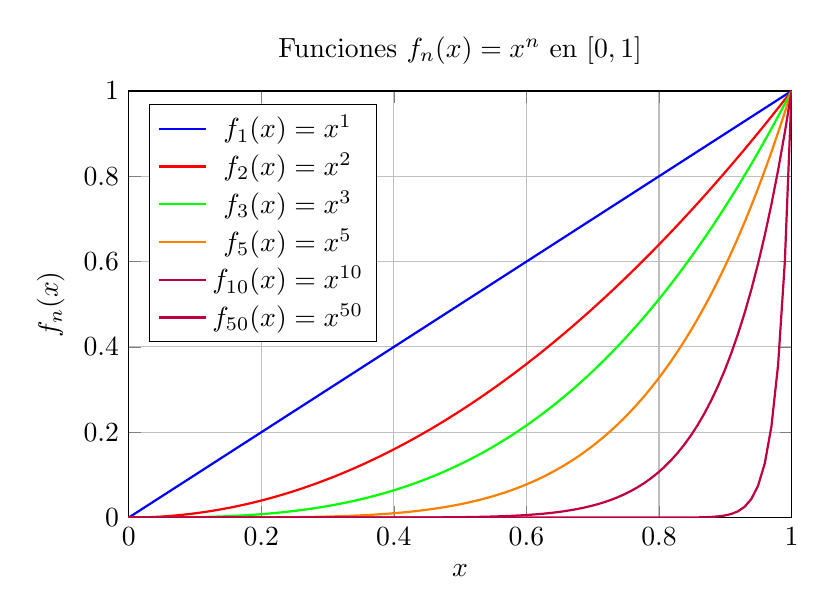
\begin{tikzpicture}
    \begin{axis}[
      width=10cm, height=7cm,
      xlabel={$x$},
      ylabel={$f_n(x)$},
      xmin=0, xmax=1,
      ymin=0, ymax=1,
      legend pos=north west,
      grid=major,
      title={Funciones $f_n(x) = x^n$ en $[0, 1]$}
    ]
      \addplot[domain=0:1, samples=100, thick, blue] {x^1};
      \addlegendentry{$f_1(x) = x^1$}

      \addplot[domain=0:1, samples=100, thick, red] {x^2};
      \addlegendentry{$f_2(x) = x^2$}

      \addplot[domain=0:1, samples=100, thick, green] {x^3};
      \addlegendentry{$f_3(x) = x^3$}

      \addplot[domain=0:1, samples=100, thick, orange] {x^5};
      \addlegendentry{$f_5(x) = x^5$}

      \addplot[domain=0:1, samples=100, thick, purple] {x^10};
      \addlegendentry{$f_{10}(x) = x^{10}$}

      \addplot[domain=0:1, samples=100, thick, purple] {x^50};
      \addlegendentry{$f_{50}(x) = x^{50}$}
    \end{axis}
  \end{tikzpicture}
\end{eg}

\begin{eg}
  $f_n: [0, 2\pi] \to \R$, $f_n(x) = cos(nx)$ no converge puntualmente pues si $x = \pi$, $f_n(\pi) = (-1)^n$ y $\nexists \lim_{n \to +\infty} f_n(\pi)$.
\end{eg}

Notemos que si $f_n: X \subset \R \to \R$ converge puntualmente a $f: X \to \R \Rightarrow (\forall \e > 0)(\exists n_0 \in \N) : |f_n(x) - f(x)| < \e$ $(\forall n > n_0)$, pero $n_0$ depende de $\e$ y de $x$. Si $\e$ está fijo puede ser que ningún $n_0 \in \N$ sirva $\forall x \in X$.

\begin{eg}
  $f_n: [0, 1] \to \R$, $f_n(x) = x^n$. Si $\e = \frac{1}{2}$ $(\forall n \in \N)(\exists x \in [0, 1)) : |f_n(x) - f(x)| \geq \e = \frac{1}{2} \iff |x^n - 0| \geq \frac{1}{2}$. En efecto pues dado $n \in \N$, $\lim_{x \to 1} x^n = 1$. 
\end{eg}

\begin{definition}[Convergencia uniforme]
  $(f_n)_{n \in \N}$ converge uniformemente a $f: X \to \R$ si $(\forall \e > 0)(\forall x \in X)(\exists n_0 \in \N) : (\forall n > n_0)$ $ |f_n(x) - f(x)| < \e$. Notamos $f_n \rightrightarrows f$.
\end{definition}

\begin{eg}
  $f_n: [0, 1] \to \R$, $f_n(x) = x^n$, $f_n(x)$ no converge uniformemente. Consideremos $f_n: [0, 1 - \delta]$, $\delta \in (0, 1) \Rightarrow$ la convergencia a $f(x) = 0$ es uniforme. En efecto, dado $\e > 0$ quiero ver que $\exists n_0 \in \N : |x^n - 0| = x^n < \e$ $\forall n > n_0$, $\forall x \in [0, 1 - \delta]$. $x^n$ es creciente entonces $0 \leq x^n \leq (1-\delta)^n$. $(1-\delta)^n \to 0$. Dado $\e > 0$, $\exists n_0 \in \N : | (1-\delta)^n - 0 | < \e$ $(\forall n > n_0) \Rightarrow |x^n - 0| \leq |(1-\delta)^n - 0| < \e$ $(\forall n > n_0)$ $(\forall x \in [0, 1-\delta]) \therefore$ la convergencia es uniforme.  
\end{eg}

\begin{definition}[Sucesión de Cauchy]
  $(f_n)_{n \in \N}$, $f_n: X \to \R$ es de Cauchy si $\forall \e > 0$, $\exists n_0 \in N : \forall n$,$m > n_0$,$\forall x \in X$, $|f_n(x) - f_m(x)| < \e$.
\end{definition}

\begin{theorem}
  Una sucesión de funciones $f_n : X \to \R$ es uniformemente convergente $\iff$ es de Cauchy.
  \begin{proof}
    Para la ida tomemos $\e > 0$, luego $\exists n_0 \in \N : |f_n(x) - f(x)| < \frac{\e}{2}$ $(\forall n > n_0)(\forall x \in X)$ por hipótesis. Luego si $n, m > n_0 \Rightarrow |f_n(x) - f_m(x)| < |f_n(x) - f(x)| + |f_m(x) - f(x)| < \e$ $(\forall x \in X)$. \\
    Para la vuelta tenemos que $\forall x \in X$ $(f_n(x))_{n \in \N}$ es una sucesión de Cauchy que converge a un límite que llamo $f(x)$. Dado $\e > 0$, $\exists n_0 \in \N : |f_n(x) - f_m(x)| < \e$ $(\forall n, m > n_0)$. $\forall x \in X$ fijado el $x$ y el $n$ tomamos $m \to +\infty \therefore |f_n(x) - f(x)| < \e$ $(\forall x \in X)(\forall n > n_0) \therefore$ la convergencia es uniforme. 
  \end{proof}
\end{theorem}

$f = \sum f_n$ es un caso particular del límite. $f : X \to \R$, $f_n: X \to \R$. $f = \lim_{n \to +\infty} S_n$, $S_n$ la suma parcial, luego $\sum f_n \rightrightarrows f \iff (\forall \e > 0)(\exists n_0 \in \N) : |S_{n+1}(x) - S_n| < \e$ $(\forall n > n_0)(\forall x \in X)$.

\begin{definition}[Convergencia normal]
  Decimos que $\sum f_n: X \to \R$ converge normalmente si $\exists (a_n)_{n \in \N} \subset \R : \sum a_n < +\infty$ y $ |f_n(x)| < a_n$ $(\forall n \in \N)(\forall x \in X)$.
\end{definition}

\begin{eg}
  $\sum_{n \geq 1} \frac{sen(n)}{n^2}$ es normalmente convergente pues $|\frac{sen(n)}{n^2}| \leq \frac{1}{n²}$ $(\forall n \in N)$ y $\sum \frac{1}{n²}$ converge.
\end{eg}

\begin{theorem}[Test de Weierstrass]
  Si $\sum f_n$ es normalmente convergente $\Rightarrow \sum |f_n|$ y $\sum f_n$ son uniformemente convergentes.
  \begin{proof}
    $X$ el dominio de todas las $f_i \Rightarrow (\forall n \in \N)(\forall p \in \N)(\forall x \in X) \Rightarrow$ \begin{equation}
      |S_{n + p}(x) - S_n(x)| = |f_{n+1}(x) + \cdots + f_{n + p}(x)|
    \end{equation}
    \begin{equation}
      \leq |f_{n+1}(x)| + \cdots + |f_{n+p}(x)|
    \end{equation}
    \begin{equation}
      \leq a_{n+1} + \cdots + a_{n+p} < \e
    \end{equation}
    Por la hipótesis de la convergencia normal $\therefore \sum f_n$ y $\sum |f_n|$ convergen uniformemente.
  \end{proof}
\end{theorem}

Notemos que la convergencia normal implica la convergencia uniforme que a su vez implica la convergencia puntual, pero el camino inverso no vale.

\begin{eg}
  $f_n: [1, +\infty) \to \R$, $f_n = \begin{cases}
    \frac{1}{x} & \text{si } x \in [n, n+1], \\
    0 & \text{caso contrario.}
  \end{cases}$
  Llamo $f: [1, +\infty) \to \R$, $f(x) = \frac{1}{x}$. Afirmo que $\sum_{n \geq 1} f_n \rightrightarrows f$. Porque $0 \leq f(x) - S_n < \frac{1}{n}$ $(\forall x \in [1, +\infty))$, pero no converge normalmente en $[1, +\infty)$, pues si fuese $f(x) \leq a_n$ $(\forall x \in [1, +\infty))$ tomando $x = n \Rightarrow \frac{1}{n} \leq a_n \Rightarrow \sum a_n = +\infty$ y no puede ser normal la serie.
\end{eg}

\begin{note}
  Sea $(f_n)_{n \in \N}$ nos preguntamos si el límite en $x$ y en $n$ son intercambiables. La respuesta en general es no.
\end{note}

\begin{eg}
  $f_n(x) = x^n$, $f(x) = \begin{cases}
    1 & \text{si } x = 1, \\
    0 & \text{si } 0 \leq x < 1. 
  \end{cases}$ \begin{equation}
    \lim_{x \to 1} (\lim_{n \to \infty} f_n(x)) = \lim_{x \to 1} f(x) = 0
  \end{equation}
  \begin{equation}
    \lim_{n \to \infty} (\lim_{x \to 1} f_n(x)) = \lim_{n \to \infty} (\lim_{x \to 1} x^n) = \lim_{n \to \infty} 1 = 1
  \end{equation}
\end{eg}

\begin{theorem}
  Sea $a$ un punto de acumulación de $X$. Si la sucesión $f_n: X \to \R$ converge uniformemente a $f: X \to \R$ y $(\forall n \in \N)(\exists \lim_{x \to a} f_n(x) = L_n) \Rightarrow$
  \begin{enumerate}
    \item $\exists \lim_{n \to \infty}$.
    \item $L = \lim_{x \to a} f(x)$.
  \end{enumerate}
  Es decir que \begin{equation}
    \lim_{n \to \infty}(\lim_{x \to a} f_n(x)) = \lim_{x \to a}(\lim_{n \to \infty} f_n(x))
  \end{equation}
  Siempre que los límites de adentro existan y el de la sucesión de funciones sea uniforme.

  \begin{proof}
    Para ver que $\exists \lim_{n \to \infty} L_n = L$. Probemos que $L_n$ es de Cauchy.
    \begin{enumerate}
      \item Dado $\e > 0$, como $f_n \rightrightarrows f$, $\exists n_0 \in \N : |f_n(x) - f_m(x)| < \frac{\e}{3}$ $(\forall n > n_0)(\forall x \in X)$. Si $m,n > n_0$, $\exists x \in X : |L_m - f_m(x)| < \frac{\e}{3}$ y $|L_n - f_n(x)| < \frac{\e}{3} \Rightarrow |L_n - L_m| \leq |L_n - f_n(x)| + |f_n(x) - f_m(x)| + |f_m(x) - L_m| < \e$.
      \item Veamos que si $f(x) = \lim_{n \to \infty} f_n$ verifica $\lim_{x \to a} f(x) = L$. Dado $\e > 0$, $\exists n_0 \in \N : |L_n - L| < \frac{\e}{3}$, $|f_n(x) - f(x)| < \frac{\e}{3}$ $(\forall n > n_0 \in \N)(\forall x \in X)$. Si $n > n_0$, como $\lim_{x \to a} f_n(x) = L_n$, $\exists \delta > 0 : 0 < |x-a| < \delta \Rightarrow |f_n(x) - L_n| < \frac{\e}{3} \Rightarrow$ si $|x-a| < \delta \Rightarrow |f(x) - L| < \e$. 
    \end{enumerate}
  \end{proof}
\end{theorem}

\begin{corollary}
  Sea $a \in X$ punto de acumulación. Si \begin{enumerate}
    \item $\sum f_n \rightrightarrows f$ en $X$
    \item $\forall n \in \N$, $\exists \lim_{x \to a} f_n(x) = L_n$
  \end{enumerate} $\Rightarrow \sum L_n < +\infty$ y $\sum L_n = \lim_{x \to a} f(x)$.
  Es decir que \begin{equation}
    \lim_{x \to a}(\sum f_n(x)) = \sum(\lim_{x \to a} f_n(x))
  \end{equation} Siempre que $\sum f_n$ sea uniformemente convergente.
\end{corollary}

Notemos que el teorema también vale si $a = +\infty$
\begin{equation}
  \lim_{n \to +\infty} (\lim_{x \to +\infty} f_n(X)) = \lim_{x \to +\infty}(\lim_{n \to +\infty} f_n(x))
\end{equation} Siempre que los límites de adentro existan y la convergencia de la sucesión de funciones sea uniforme. La demostración queda como ejercicio.

\begin{theorem}
  Si $f_n \rightrightarrows f$ y todas las $f_n$ son continuas en $a \in X \Rightarrow f$ es continua en $a$.
  \begin{proof}
    Si $a$ es punto aislado es inmediato. Si $a \in X^{\prime} \Rightarrow$ \begin{equation}
      \lim_{x \to a} f(x) = \lim_{x \to a}(\lim_{n \to \infty} f_n(x)) 
    \end{equation}
    \begin{equation}
      = \lim_{n \to \infty}(\lim_{x \to a} f_n(x)) = \lim_{n \to \infty} f_n(a) = f(a)
    \end{equation}
  \end{proof}
\end{theorem}

Si el límite de $(f_n)_{n \in \N}$ no es continuo y las funciones de la sucesión sí, el límite no puede ser uniforme. Por otro lado que el límite sea continuo tampoco alcanza para que la convergencia sea uniforme.

\begin{definition}[Convergencia monótona]
  Decimos que $(f_n)_{n \in \N}$ converge monótonamente a $f$, si $(\forall x \in X)$ la sucesión $(f_n)_{n \in \N}$ es monótona y $f_n(x) \to f(x)$.
\end{definition}

\begin{theorem}
  Sea $X \subset \R$ compacto. Si una sucesión de funciones continuas $f_n: X \to \R$ converge monótonamente a una función continua $f: X \to \R \Rightarrow$ la convergencia es uniforme.
  \begin{proof}
    Dado $\e > 0$, sea $K_n = \{ x \in X : |f_n(x) - f(x)| \geq \e \}$ $(\forall n \in \N)$. Como $f_n$, $f$ son continuas, $K_n$ es cerrado de $X \Rightarrow K_n$ es compacto $(\forall n \in \N)$. Afirmo que como $(f_n)$ es monótona, $K_1 \supset K_2 \supset K_3 \supset \cdots$ si $f_1 < f_2 < \cdots < f \Rightarrow -f_1 > -f_2 \Rightarrow f - f_1 > |f - f_2| \Rightarrow K_1 \supset K_2 \cdots$. Y si, $f_1 > f_2 > \cdots > f \Rightarrow f_1 - f > |f - f_2| \Rightarrow K_1 \supset K_2 \cdots$. Pero además debe ser $\bigcap_n K_n \neq \varnothing$ porque si no $|f(x) - f_n(x)| \geq \e$ $(\forall n \in \N)$ absurdo $\Rightarrow \exists n_0 \in \N : K_{n_0} = \varnothing \Rightarrow K_n = \varnothing$ $(\forall n > n_0) \Rightarrow |f(x) - f_n(x)| < \e$ $(\forall n > n_0)(\forall x \in X)$.
  \end{proof}
\end{theorem}

\begin{corollary}
  Una serie convergente de funciones no negativas, continuas, definidas en un compacto es uniformemente convergente $\iff \sum f_n(x)$ es continua en un compacto.
  \begin{proof}
    $S_n = f_1 + \cdots + f_n$ es una sucesión monótona pues son no negativas.
  \end{proof}
\end{corollary}

\section{Integración de sucesiones de funciones}

\begin{theorem}
  Si $f_n: [a, b] \to \R$ son funciones integrables que convergen uniformemente a $f: [a, b] \to \R \Rightarrow$ es integrable y vale que $\int_a^b f(x) dx = \lim_{n \to +\infty} \int_a^b f_n(x) dx$.
  \begin{proof}
    Sean $D_n$ y $D$ los conjuntos de discontinuidad de $f_n$ y $f$. Si $x \notin D_n$ $(\forall n \in \N) \Rightarrow x \notin D$, pues el límite uniforme es continuo en los puntos de discontinuidad. Luego $D \subseteq \bigcup_n D_n$ Como $|D_n| = 0$ $(\forall n \in \N)$, pues son integrables, tenemos que $|D| = 0 \Rightarrow f$ es integrable. Ahora, dado $\e > 0$, $\exists n_0 \in \N : |f_n(x) - f(x)| < \frac{e}{b-a}$ $(\forall x \in [a, b])(\forall n > n_0)$. Luego $(\forall n > n_0)$ \begin{equation} |\int_a^b f(x) dx - \int_a^b f_n(x) dx| \leq \int_a^b |f(x) - f_n(x)|dx < \frac{\e}{b-a} \cdot (b-a) = \e
    \end{equation}
    Es decir que $\int_a^b \lim_{n \to +\infty} f_n(x) dx = \lim_{n \to +\infty} \int_a^b f_n(x) dx$.
  \end{proof}
\end{theorem}

\begin{corollary}
  Si $\sum f_n \rightrightarrows f$ y las $f_n$ son integrables $\Rightarrow$ la suma es integrable y $\int_a^b \sum f_n = \sum \int_a^b f_n$ en otras palabras, la serie se puede integrar término a término.
\end{corollary}

\begin{note}
  Si $f_n: [a, b] \to \R$ son integrables y convergen puntualmente a $f$ en $[a, b]$ puede pasar que $f$ no sea integrable por ejemplo si $\Q \cap [a, b] = \{r_1, \cdots\}$ y 
  \begin{equation}
    f_n(x) = \begin{cases}
      1 & \text{si } x \in \{r_1, \cdots, r_n\}, \\
      0 & \text{caso contrario}.
    \end{cases}
  \end{equation}
  Luego $f(x) = \begin{cases}
    1 & \text{si } x \in \Q \cap [a, b], \\
    0 & \text{caso contrario}.
  \end{cases} \Rightarrow f_n \to f \text{ en } [a, b]$, cada $f_n$ es integrable, pero $f$ no lo es.
\end{note}

\begin{note}
  $f_n \to f$ en $[a, b]$, $f_n$ y $f$ son integrables, pero $\lim_{n \to \infty} \int_a^b f_n \neq \int_a^b f$. Por ejemplo si $f_n: [0, 1] \to \R$, $f_n(x) = \begin{cases}
    (n+1) x^{n+1} & \text{si } x \in [0, 1), \\
    0 & \text{si } x = 1.
  \end{cases}$ Luego si $f: [0, 1] \to \{0\}$, $f(x) = 0 \Rightarrow f_n \to f$, pero $\int_0^1 f_n(x) dx = 1 \neq 0 = \int_0^1 f(x) dx$. 
\end{note}
